% Copyright 2008 by Marc de Falco
%
% This file may be distributed and/or modified
%
% 1. under the LaTeX Project Public License and/or
% 2. under the GNU Public License.
%
\documentclass[10pt,a4paper]{article}
\usepackage[fancy,color=orange]{tikz-inet}
\usetikzlibrary{calc}
\usepackage{ifthen}

\usepackage{fancyvrb}
\usepackage{a4wide}
\usepackage{pgffor}

\newenvironment{outputverbat}{%
    \VerbatimEnvironment\begin{VerbatimOut}{\jobname.tmp}}
    {\end{VerbatimOut}}
\newcommand{\code}[1][0.5]{
    \fbox{
    \begin{minipage}{#1\textwidth}
      \VerbatimInput[gobble=4,fontsize=\footnotesize]{\jobname.tmp}
    \end{minipage}
    }
}
\newcommand{\picturefancy}
    {\begin{tikzpicture}\input{\jobname.tmp}\end{tikzpicture}}
\newcommand{\picturenofancy}
    {\begin{tikzpicture}\inetnofancy\input{\jobname.tmp}%
    \inetfancy\end{tikzpicture}}
\newenvironment{exampleH}{\VerbatimEnvironment\begin{outputverbat}}
    {\end{outputverbat} 
    \begin{center}
    \begin{tabular}{c|cc}\picturefancy & \picturenofancy & \code\end{tabular}
    \end{center}}
\newenvironment{exampleHv}{\VerbatimEnvironment\begin{outputverbat}}
    {\end{outputverbat} 
    \begin{center}
    \begin{tabular}{c}
        \begin{tabular}{r|l}
            \picturefancy & \picturenofancy 
        \end{tabular}
        \\ \hline \\ \code[1]\end{tabular}
    \end{center}}
\newenvironment{exampleVv}{\VerbatimEnvironment\begin{outputverbat}}
    {\end{outputverbat} 
    \begin{center}
    \begin{tabular}{rl}
        \begin{tabular}{c}
        \picturefancy \\ \hline \\  \picturenofancy
        \end{tabular}
        & \code
    \end{tabular}
    \end{center}}

\begin{document}

\title{The package \textsf{tikz-inet}}
\author{Marc de Falco}
\maketitle

\begin{abstract}
    The purpose of this package is to extend tikz
    with some simple macros in order to draw interaction
    nets.
\end{abstract}

\section*{Changelog}
\newcommand{\changeitem}[2]{\item \textbf{#1} \textit{#2}}
\begin{itemize}
    \changeitem{0.1}{initial release}
\end{itemize}

\section*{TODO}
\begin{itemize}
    \item add support for proofnets
\end{itemize}

\section{Installation}
Install this package in your ressource directory or the root of your 
document directory.

This package obviously needs tikz and pgf, but \textbf{this package needs
the version, at least, 2.0 of them}.

\section{Usage}
\subsection{Loading the package}
The command to load the package is the usual 

\verb+\usepackage[<+\emph{options}\verb+>]{tikz-inet}+

where \emph{options} are a comma separated list of keys ranging in

\begin{description}
    \item[fancy] Select a fancier style suitable for talks but
        likely to frighten referees
    \item[color=] The global color used by the fancy style, must
        be xcolor compliant color
    \item[angle=] The default orientation of cells, in degrees (default to $0$, that is a cell pointing downward)
\end{description}

\subsection{Cell nodes}
The cells are displayed using the internal node system of tikz.
A special shape \emph{cellule} is inherited from the tikz shape 
isosceles triangle, thus sharing the original anchors.

A macro is defined to encapsulate the node creation.

\verb+\inetcell[+\emph{tikz display keys}\verb+](+\emph{node name}%
\verb+){+\emph{symbol}\verb+}[+\emph{angle}\verb+]+

Every parameter is optional but the symbol.

\begin{description}
    \item[symbol] The symbol of the cell, that is the text displayed
        in the center of the cell. This text is not assumed to be
        in math mode.
    \item[node name] This is the name of the node that will be
        used for referencing it or connecting wires. This name
        default to the symbol, which is a convenient way to make simple
        drawings, this can lead to some error as soon as the symbol
        is not simple, like a math text.
    \item[angle] The angle of the principal port of the cell,
        defaults to $0$ which means that the cell has a downward
        orientation with the principal port on the right.

        Special values $U,D,L$ and $R$ are defined for up, down, left and right
        orientation of the cell.
    \item[tikz display keys] This additional display keys are 
        appended to the one used by the package and given to the
        node construction. As it is appended after, it can be used to 
        redefine all display options.

        A special key \verb+arity+ allows to define arity based anchors
        for ports. This is not really useful in most cases as the
        three predefined anchors are more likely to suit your need.
\end{description}

When using this macro a lot of parameters are given to tikz, one of
them is the current cell display style. More on this can be found later.

\subsubsection{Ports}
Some anchors are named in order to reflect ports of the cell:
\begin{description}
    \item[pal] the apex of the triangle, where lies the principal port
    \item[middle pax] an auxiliary port aligned with the principal port
    \item[left pax, right pax] auxiliaries ports on each side of the opposite
        edge of the apex
    \item[pax $n$, $1 \le n \le arity$] numbered auxiliary ports associated
        with the arity key.
\end{description}

Each anchor has a sibling a bit off the cell, it allows nice curving when
branching wires. To get this special anchor, just add \verb+above+ to the 
other ones: e.g. \verb+above middle pax+

\begin{center}
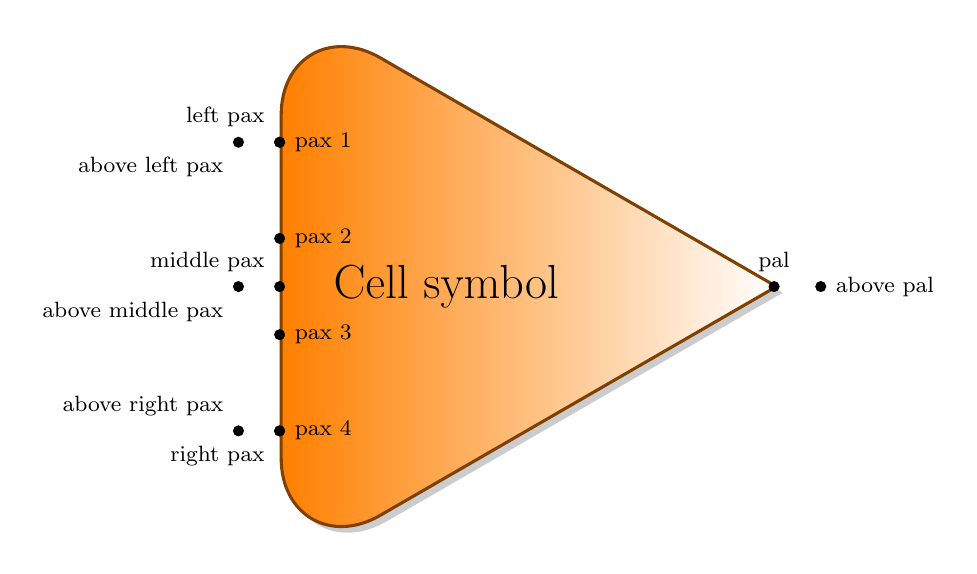
\begin{tikzpicture}
    \LARGE
    \inetcell(c){Cell symbol}[90]
    \fill (c.pal) circle (2pt) 
        node[above]{\footnotesize pal};
    \fill (c.above pal) circle (2pt) 
        node[right]{\footnotesize above pal};
    \fill (c.left pax) circle (2pt) 
        node[above left]{\footnotesize left pax};
    \fill (c.above left pax) circle (2pt) 
        node[below left]{\footnotesize above left pax};
    \fill (c.middle pax) circle (2pt) 
        node[above left]{\footnotesize middle pax};
    \fill (c.above middle pax) circle (2pt) 
        node[below left]{\footnotesize above middle pax};
    \fill (c.right pax) circle (2pt) 
        node[below left]{\footnotesize right pax};
    \fill (c.above right pax) circle (2pt) 
        node[above left]{\footnotesize above right pax};
    \foreach \x in {1,...,4} {
        \fill (c.pax \x) circle (2pt)
            node[right]{\footnotesize pax \x};
    }
\end{tikzpicture}
\end{center}

\subsection{Wires}
Wires macros help connecting ports by taking into account the current
wire display style and dealing implicitly with the \emph{above} anchors.
The wires are displayed on a layer below the main one, so cells are always
on top of layers. To change this you have to use \verb+\pgfsetlayers+.

\verb+\inetwire[+\emph{tikz extra display keys}\verb+](cell1.port1)(cell2.port2)+

The arguments are self-explanatory: this wire will connect the port \verb+port1+
of \verb+cell1+ with the port \verb+port2+ of \verb+cell2+. It uses the current
wire style.

\verb+\inetloop[+\emph{tikz extra display keys}\verb+]+ 

draws a loop, that is a circle with the current wire style

\verb+\inetwirecoords[+\emph{tikz extra display keys}\verb+](A)(B)+ 

draws a wire from node A to node B with the current wire style. It's useful
to add extra wires non linking cell ports while using the current wire style.

\verb+\inetwirefree[+\emph{tikz extra display keys}\verb+](cell.port)+

draws a wire from \verb+port+ of \verb+cell+ to \verb+above port+
of the same cell, with
the current wire style. It allows fast declaration of free ports.

\subsection{Boxes}
Boxes uses the current box style when being displayed, they lie on a 
layer below the wire layer.

\verb+\inetbox[+\emph{tikz extra display keys}\verb+]{+\emph{space 
separated list of cells in the box}\verb+}(+\emph{box node name}+\verb+)+
display a box containing the given cells

\verb+\inetprombox[+\emph{tikz extra display keys}\verb+]{+\emph{space 
separated list of cells in the box}\verb+}(+\emph{promotion cell 
node name}+\verb+)+: display a box and add a promotion cell below it, 
the name of the box is \verb+bname+ where \verb+name+ is the name
of the promotion cell.



\subsection{Other macros}
\verb+\inetnofancy+, \verb+inetfancy+: hotswap the current display style

\verb+\inetcellstyle+,\verb+\inetwirestyle+,\verb+\inetboxstyle+: get
the currently used style for each type of drawing. \textbf{Don't renew this
command to define your own style!}

\verb+\inetcolor+: the current color for the fancy style, also passed
as an argument of the non fancy style.

If you want to call a style you have to give an argument, unless you have
redefined the fancy styles to not use it. For a cell like element you have
to give the key \verb+\inetcellstyle=\inetcolor+.

\subsubsection{Tikz styles}
This package define six styles :
\begin{itemize}
    \item \emph{cellstyle} and \emph{fancycellstyle}
    \item \emph{wirestyle} and \emph{fancywirestyle}
    \item \emph{boxstyle} and \emph{fancyboxstyle}
\end{itemize}
You can redefine this styles as for any other tikz styles with the
command:

\verb+\tikzset{+\emph{the style name}\verb+/.style={+\emph{tikz display keys}\verb+}}+

\section{Examples}
\subsection{Basic}
    All examples are shown with the \textsf{fancy} key on the left.

    \begin{exampleH}
    \inetcell{A}
    \end{exampleH}

    \begin{exampleVv}
    \matrix[row sep=0.5cm]{
        \inetcell{A} & & \inetcell{B} \\
        & \inetcell{C} & \\
    };
    \inetwirefree(A.middle pax)
    \inetwirefree(B.middle pax)
    \inetwirefree(C.pal)
    \inetwire(A.pal)(C.right pax)
    \inetwire(B.pal)(C.left pax)
    \inetbox{(A) (B)}(b)
    \end{exampleVv}

\subsection{Style variations}

    \begin{exampleVv}
    \matrix{
    \inetcell{A} & 
    \inetcell[fancycellstyle=green]{B} \\
    \inetcell[bottom color=green]{C} &
    \inetcell[draw=black]{D} \\
    \inetcell[very thick]{E} &
    \inetnofancy \inetcell{F} \inetfancy \\
    };
    \end{exampleVv}

\subsection{Special cases}
    \begin{exampleVv}
    \inetcell{A}
    \inetprombox{(A)}(pa)
    \inetcell[at=(bpa.east),right=5pt]{B} 
    \inetwire(B.middle pax)(A.middle pax)
    \inetprombox{(bpa)(pa)(B)}(p)
    \inetwire(A.pal)(pa.middle pax)
    \inetwirefree(pa.pal)
    \inetwirefree(p.pal)
    \inetwire(B.pal)(p.middle pax)
    \end{exampleVv}

    \begin{exampleVv}
    \newcount\angle
    \foreach \x in {1,...,12} {
        \pgfmathsetcount{\angle}{360*\x/12+90}
        \inetcell[\inetcellstyle=green!\x0,
            at=(\the\angle-90:1.5cm)]
            (c\x){A}[\angle]
    }
    \end{exampleVv}

    \begin{exampleHv}
    \newcount\angle
    \newcount\order
    \order=10
    \newcount\arity
    \pgfmathsetcount{\arity}{\order-1}
    \foreach \x in {1,...,\order} {
        \foreach \y/\symbol in {0/!,1/?} {
            \pgfmathsetcount{\angle}
                {(180*(2*\x+\y))/\order+90}
            \inetcell[at=(\the\angle-90:\the\order*1.8ex),
                arity=\order-1](c\y\x){\symbol}[\angle]
            \inetwirefree(c\y\x.pal)
        }
    }
    
    \newcount\nextcell
    \newcount\nextport
    \newcount\depth
    \foreach \x in {1,...,\order} {
        \foreach \y in {1,...,\arity} {
            \pgfmathsetcount{\nextcell}
                {mod(\x+\y-1,\order)+1}
            \pgfmathsetcount{\nextport}
                {\arity-\y+1}
            \pgfmathsetcount{\depth}{(\x-1)*100/\order}
            \inetwire[\inetwirestyle=\inetcolor!\the\depth!black]%
                (c0\x.pax \y)(c1\the\nextcell.pax \the\nextport)
        }
    }
    \end{exampleHv}

\end{document}
